\documentclass{article}

\usepackage{marvosym}
\usepackage{amsmath}
\usepackage{amsfonts}
\usepackage{graphicx}
\usepackage{babel}
\usepackage{algorithm}
\usepackage{algpseudocode}
\usepackage{hyperref}

\graphicspath{{images/}}

\renewcommand\refname{Viri}


\author{Gašper Terglav}
\date{22. maj 2024}
\title{Najkrajša pot z odstranljivimi ovirami}


\begin{document}


\maketitle


\section*{Predstavitev problema}

Problem je posplošitev klasične verzije, v kateri se oviram lahko samo izogibamo. V $\mathbb{R}^2$ imamo dve točki s in t ter iščemo najkrajšo evklidsko pot med njima. Ovire v ravnini so konveksni večkotniki, vsak od njih ima ceno $c_i > 0$. Če imamo na voljo $C$ ''denarja'', katere ovire se splača odstraniti, da dosežemo najkrajšo pot? V resničem življenju lahko npr.\ načrtovalci mest spremenijo cestno omrežje, da dosežejo boljšo pretočnost in tako odstranijo ovire za neko ceno. Še en primer omenjen v članku so skladišča v katerih delajo roboti. Kako spremeniti postavitev ovir v skladišču, da se roboti hitreje premikajo okoli? 

Preprost primer, na katerem so ovire s cenami, začetek, konec ter proračun, je prikazan na sliki \ref{fig:errPr1}.

\begin{figure}[h]
    \centering
    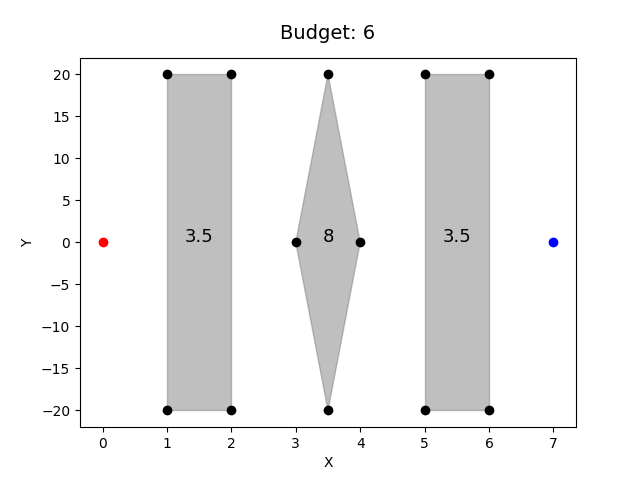
\includegraphics[width=0.65\textwidth]{err1.png}
    \caption{Primer problema.}
    \label{fig:errPr1}
\end{figure}


Zanima nas ali obstaja pot dolžine $L$ in cene $C$ med začetkom in koncem? Ta problem je na žalost NP-težek, zato se bomo za polinomski čas morali zadovoljiti z algoritmom, ki ima neko napako vsaj v ceni. Še pred algoritmi iz članka pa je treba narediti t.~i.\ ''viability graph'' za naš problem.



% \subsection*{NP-težkost}

% Naš problem je NP-težek. To pokažemo z redukcijo na problem PARTITION, ki je NP-poln. Pri tem problemu imamo množico $A = \{a_1, a_2, ..., a_n\}$ pozitivnih celih števil. Vprašanje je, ali lakho $A$ razdelimo v množici $A_1$ in $A_2$, tako da je $W(A_1) = W(A_2) = \frac{1}{2}W(A)$, kjer je $W(S)$ vsota vseh elementov v $S$. Redukcijo dosežemo tako, da med točki $s$ in $t$ postavimo $n$ ovir, tako da je cena odstranitve enaka dolžini, za katero se pot podaljša, če ovire ne odstranimo. Če obstaja pot med s in t dolžine $\frac{1}{2}W(A) + \lVert s - t \rVert$ , kjer imamo $\frac{1}{2}W(A)$ proračuna za odstranitev ovir, potem smo našli razdelitev $A$ na dva enaka dela. Ovire, ki smo jih odstranili damo v eno možico, ostale pa v drugo.  

\section*{Algoritmi}

\subsection*{Viability graph}

Začnimo s pomembnima opazkama o obnašanju najkrajše poti. Če bo šla naša pot skozi oviro, bo zaradi konveksnosti sekala samo dve stranici večkotnika. Smer bo pot spremenila samo v ogliščih večkotnikov. Tako bomo lahko problem prevedli na iskanje najkrajše poti v grafu, katerega vozlišča so vsa oglišča ovir ter točki $s$ in $t$. Označimo ta graf z $G = (V, E)$, kjer $(u,v) \in E$, če je vsota cen vseh ovir, ki jih prečka daljica $\overline{uv}$, manjša ali enaka od našega proračuna $C$. Vsaka povezava v grafu ima dva parametra, dolžino in ceno. 

Najprej sem se konstrukcije lotil naivno. Za vsak par točk sem za vsako oviro pogledal, če jo pot seka. Ta pristop ima časovno zahtevnost $O(n^3)$. Je pa tudi veliko robnih primerov, ki otežijo implementacijo. Trenutna implementacija ima problem, ko je na poti med ogliščema še tretje oglišče. Če sta drugo in tretje oglišče del iste ovire in gre pot po njeni notranjosti, tega nisem znal na lep način zaznati. Tako bi imela ta povezava premajhno ceno. Implementacija je v datoteki ''viabilityGraph.py''

Viabilty graph je v resnici posplošitev konstrukcije z imenom angleškim imenom visibility graph, s katerim se rešuje osnovno verzijo problema, kjer je $C = 0$. O tej verziji je več literature, s katero sem si lahko pomagal. Zato sem izgradnjo visibility grapha iz knjige~\cite{BCKO} v poglavju $15$ posplošil na viability graph. 
Na vsakem koraku pri konstrukciji izberemo novo oglišče $v$. Ugotoviti moramo, do katerih oglišč lahko iz $v$ pridemo s ceno največ $C$. Pri naivnem pristopu smo oglišča pregledali ''kakor so padla''. Sedaj pa jih hočemo v nekem pametnem vrstnem redu, da bomo lahko nekaj informacij o oglišču uporabili pri naslednjem. Predstavljajmo si poltrak $p$, ki ima izhodišče v $v$ in naredi en krog v smeri urinega kazalca. Oglišča bomo pregledali v vrstnem redu, ki ga določa ta sprehod poltraka (ang.\ plane sweep). Če $p$ oglišča seka istočasno, imajo prednost tista, ki so bližje $v$. Robove ovir, ki jih $p$ seka, bomo shranili v dvojiško drevo, kar omogoča hitrejše dodajanje in brisanje. Psevdokoda je v Algorithm \ref{alg:visibleFromV}.

\begin{algorithm}
    \caption{Vrnem seznam oglišč, ki jih lahko dosežemo iz $v$}
    \label{alg:visibleFromV}
    \begin{algorithmic}[1]
        \State Uredimo preostala oglišča glede na kot, ki ga daljica med ogliščem in $v$ naredi s pozitivno x-osjo.
        \State  Dodamo v drevo vse robove, ki jih $p$ seka. Prvi rob je tisti, ki ga poltrak najprej seka.
        \State $W$ = [ \ ]
        \For{ $w_i$ v urejenih ogliščih } 
        \If{(cena poti med $v$ in $w_i$) $\leq C$}
            \State Dodamo $w_i$ v $W$.
        \EndIf
        \State Zavrtimo poltrak $p$, da gre sedaj še skozi $w_i$.
        \State Odstranimo iz drevesa robove ovir, ki se končajo v $w_i$ ter ležijo nad $p$.
        \State Dodamo v drevo robove, ki se končajo v $w_i$ in ležijo pod njim.
        \EndFor
        \State \Return $W$
    \end{algorithmic}
\end{algorithm}

Ta algoritem poženemo za vsako oglišče, ki ga imamo in tako lahko sestavimo naš viability graph. Potrebujemo pa še funkcijo, ki nam v 5. koraku izračuna ceno poti. Kot argument ji moramo podati točke $v$, $w_i$, $w_{i-1}$ ter ceno poti $vw_{i-1}$ in še naše dvojiško drevo ter vse ovire. Ključno je, da če $w_i$ in $w_{i-1}$ ležita na isti premici, lahko uporabimo to kar vemo o $w_{i-1}$.

Ta funkcija z imenom \emph{viable} nato za vsak $w_i$ pregleda dvojiško drevo in sešteje cene vseh ovir, ki jih $vw$ seka. Že to je počasneje kot v verziji problema, ko je $C = 0$. Tam nas večino časa zanima samo rob z najmanjšim ključem v drevesu, saj je ta najbližje $v$. Če obstaja in seka $\overline{vw_i}$ potem $w_i$ seveda ni viden. Celotno drevo pregledujemo tam samo, če sta $w_i$ in $w_{i-1}$ kolinearna in je $w_{i-1}$ viden. In tudi v tem primeru iščemo samo do prvega presečišča. Drugi problem je, da moramo vsakič na začetku preveriti, ali sta $v$ in $w_i$ del iste ovire. V trenutni implementaciji se tega lotim naivno, kar ima zahetvnost $O(n)$. Zaradi tega je zahtevnost celotnega algoritma skupaj spet $O(n^3)$, kljub temu da je zahtevnost tistega v \cite{BCKO} le $O(n^2 \log n)$. Prvi korak v izboljšavi algoritma je torej nov algoritem, ki preveri če sta dve oglišči del iste ovire. Implementacija se nahaja v datoteki \emph{sweepViabilityGraph.py}. Rezultat algoritma, uporabljenega na našem problemu vidimo na sliki \ref{fig:errG1}.

\begin{figure}[h]
    \centering
    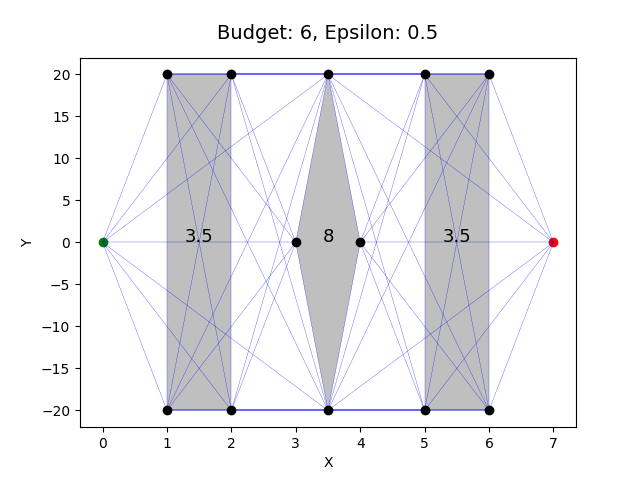
\includegraphics[width=0.65\textwidth]{errGraph1.png}
    \caption{Viability graph.}
    \label{fig:errG1}
\end{figure}

 
\subsection*{Preprost algoritem v polinomskem času z napako v ceni}

Ker imamo viability graph $G = (V,E)$, lahko končno začenmo z vsebino članka. Glavni problem je, da imajo povezave v $G$ dva parametra: ceno in dolžino.
Graf bi radi modificirali tako, da bi na novem grafu samo pognali Dijkstra algoritem in dobili rešitev, zato hočemo nekako odstraniti cene iz povezav. 

Naj bo  zaradi preprostosti $K = min(\frac{C}{min_i \ c_i}, h)$, kjer je $h$ število ovir, $c_i$ pa njihove cene ter $\sum c_i = C$. Delimo vse cene z $K/C$, da je naš proračun za ovire na tako enak $K$. Potem naredimo $ \lceil{\frac{2K}{\epsilon}}\rceil + 1$  kopij vsakega vozličša v grafu $G$ in jih označimo z $v_0, v_{\epsilon/2}, v_{\epsilon}..., v_K$. Za vsak rob $(u, v) \in E$ s ceno $c$ in za vsak $0 \le i \le \lceil{\frac{2K}{\epsilon}}\rceil $, dodamo rob $(u_{i \epsilon/2}, v_{j \epsilon/2})$, kjer je $j\le\lceil{\frac{2K}{\epsilon}}\rceil$ največje celo število, da velja $j\frac{\epsilon}{2}
 \le i \frac{\epsilon}{2} + c$. Dolžina povezav je enaka kot v originalnem grafu. Tako smo ceno zakodirali v vozlišča. Indeks v vozlišču nam pove, koliko smo plačali na poti do sedaj. Na koncu dodamo še novi vozlišči $s$ in $t$, ter vsakega od njiju povežemo z vsemi njunimi kopijami. Te povezave imajo dolžino $0$. Ker imajo povezave samo še dolžino, lahko sedaj za iskanje najkrajše poti uporabimo Dijkstro. Novi graf ima $O(|V|K/\epsilon)$ vozlišč in $O(|E|K/\epsilon)$ robov. Dijkstra  je  časovno najbolj zahtevna stvar, zato je časovna zahtevnost celotnega algoritma enaka $O(\frac{K}{\epsilon}(|E| + |V|\log\frac{|V|}{\epsilon}) )$. Če je $n$ število vseh oglišč ovir, je to v najboljšem primeru $\Omega(\frac{n^3}{\epsilon})$. Cena poti, ki jo vrne ta algoritem, je največ $(1 + \epsilon)C$. Implementacija kopiranja grafov je v datotekah za izgradnjo viability graphov, saj je v obeh primerih razred $Graph$ malo drugače definiran. Dijkstra pa je v $dijkstra.py$.

 Tako lahko končno najdemo najkrajšo pot pri našem problemu, prikazano na sliki \ref{fig:errP1}.

 \begin{figure}[h]
    \centering
    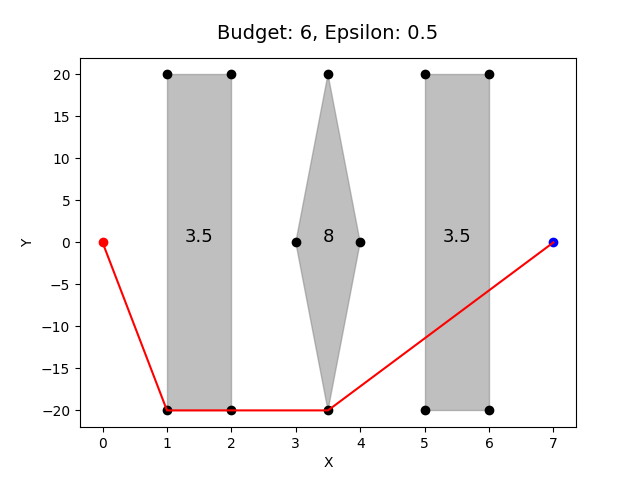
\includegraphics[width=0.65\textwidth]{errPath1.png}
    \caption{Najkrajša pot z $\epsilon = 0.5$.}
    \label{fig:errP1}
\end{figure}

V svoji implementaciji zaradi preprostosti ne naredim $2/\epsilon$ kopij temveč samo $1/\epsilon$. Posledično bo cena najkrajše poti manjša od $(1 + 2\epsilon)C$. Čeprav je naš primer zelo preprost, se napaka pojavi če izberemo $\epsilon > 0.5$, kot vidimo na sliki \ref{fig:errP05}.

\begin{figure}[ht]
    \centering
    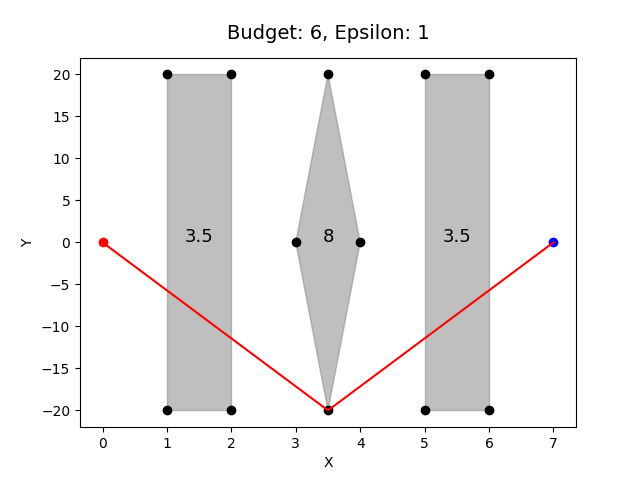
\includegraphics[width=0.65\textwidth]{errPathEps1.png}
    \caption{Najkrajša pot z $\epsilon = 1$.}
    \label{fig:errP05}
\end{figure}




\subsection*{Hitrejši algoritem}

Za večjo hitrost bomo morali modificirati graf $G$. Pravzaprav hočemo zmanjšati število povezav v grafu, na katerem na koncu poženemo Dijsktro. V zameno pa je tukaj lahko napaka $(1+\epsilon)$ tudi pri dolžini poti. Algoritem ima dva dela. Najprej konstruiramo nov graf $H = (X,\Gamma)$, ki bo imel manj povezav kot $G$. Ta algoritem ima časovno zahtevnost $O(\frac{nh}{\epsilon^2}\log n \log \frac{n}{\epsilon})$. 
% kar je približno za potenco $n$ manj kot prejšnji algoritem.

\subsubsection*{Konstrukcija grafa $H$}

Začeli smo z grafom $G = (V,E)$. Za $H = (X,\Gamma)$ bo veljalo $|X|, |\Gamma| = O(n \log n)$ in $V \subseteq X$. Označimo razdaljo med ogliščema $v,u$ v grafu $G$ z $d_G(v,u)$. Potem bo za vsak par $v,u \in G$ veljalo  $d_G(v,u) \leq d_H(v,u) \leq \sqrt{2}d_G(v,u)$. Da bomo lahko zmanjšali število povezav, bomo morali, kakor se sliši čudno, povečati število vozlišč. Potegnili bomo navpično premico, ki naša oglišča razdeli na dva približno enaka dela in nato dodali v graf projekcije vozlišč na premico. To bomo rekurzivno ponovili na obeh polovicah in tako naprej rekurzivno. Nato vse še enkrat z vodoravnimi premicami. Potem bomo dodali povezave, večina jih bo oblike (vozlišče, njegova projekcija). Tako bodo poti v grafu sestavljene bolj iz vodoravnih in navpičnih segmentov. Celoten postopek je opisan v Algorithm \ref{alg:sparseGraph}.

\begin{algorithm}
    \caption{Dobimo graf $H$ z manj povezavami}
    \label{alg:sparseGraph}
    \begin{algorithmic}[1]
        \State Naj bo $x_m$ mediana za $x$-koordinate točk v $V$. 
        \State  Naj bo $l_v: \ x = x_m$ navpična premica, ki razdeli $V$ na levo polovico $V_l$ in desno $V_d$.
        \For{ $v \in V$} 
            \State Dobimo projekcijo $v' = (x_m,v_y)$
            \If {cena poti $\overline{vv'} \leq C$}
                \State Dodamo $v'$ v $X$ in $(v,v')$ v $\Gamma$
            \EndIf
            \State Naj bo $s'$ prvi rob ovire s pozitivnim naklonom, ki seka $\overline{vv'}$. 
            \If{$s'$ seka $l_v$} 
                \State Dodali bomo ''obhodna'' vozlišča in povezave v $H$.
                \State Označimo presečišče $\overline{vv'}$ in $s'$ z $v_1$ in presečišče $s'$ in $l_v$ z $v_2$. 
                \State Dodamo ti dve točki v $X$ ter povezavi $(v,v_1)$ in $(v_1,v_2)$ v $\Gamma$.
            \EndIf
            \State Ponovimo postopek za prvi $s'$ z negativnim naklonom.
            \State Recimo točkam na premici $l_v$ Steinerjeve točke.
            \For{$w, w'$ sosednji Steinerjevi točki}
                \State Če je cena $\overline{ww'} \leq C$, dodamo $(w,w')$ v $\Gamma$.
            \EndFor
        \EndFor
        \State Rekurzivno ponovimo na množicah $V_l$ in $V_d$.
        
        \State Ponovimo vse zgoraj, le tokrat z mediano $y_m$ za $y$-koordinate  in premico $l_h: \ y_m = y$.
        \State Dodamo v $\Gamma$ še robove ovir.
    \end{algorithmic}
\end{algorithm}

Da izvedemo celoten algoritem potrebujemo dve stvari. Za vsak par $vv'$ moramo poiskati prvi rob z pozitivnim in prvi rob negativnim naklonom, ki seka $\overline{vv'}$. Za vsako povezavo, ki jo dodamo v graf, moramo izračunati njeno ceno. Za razliko od grafa $G$, bodo tukaj vse povezave, ki niso na povrišini ovir, vodoravne ali navpične. Zato sem si pomagal s člankom \cite{SnT} ter implementiral verzijo binarnih dreves (ang.\ persistent binary search tree), ki omogoča rešitev naslednjega problema: za vertikalno daljico najde vse večkotnike, ki jih daljica seka. Angleški izraz bom prevedel na časovna drevesa.

Osnovni namen teh dreves je rešiti problem iskanja lokacije točke v ravnini (ang.\ planar point location). Če imamo delitev ravnine na večkotnike nas potem za neko točko zanima, kateri večkotnik jo vsebuje. Problema se v članku lotijo tako, da potegnejo navpično premico čez vsako oglišče večkotnika. Tako razdelimo ravnino na trakove. Za lokacijo točke potem potrebujemo le dve binarni iskanji: najprej poiščemo trak, ki točko vsebuje, nato pa v traku najdemo še najbližji rob večkotnika pod točko. Lahko bi za vsak trak naredili eno dvojiško drevo, vendar to porabi več prostora kot naša rešitev. Namesto veliko dreves bi lahko imeli eno drevo, ki se spreminja skozi čas in omogča, da dostopamo do starejših verzij. Ravno to omogočajo časovna drevesa. Želene lastnosti dosežemo s kopiranjem poti (ang. path copying). Če imamo drevo ob času 0 in dodamo nov element ob času 1, potem naredimo kopije vseh vozlišč, ki so na poti od korena do novega vozlišča in označimo čas njihovega nastanka. Če torej želimo pogledati verzijo drevesa v času $t$, samo začemo v korenu, ki je nastal ob času $t$ in normalno hodimo po drevesu. Ampak to spet porabi veliko prostora, saj kopiramo veliko vozlišč. Glavna ideja članka je, da dopustimo vozliščem $2 + k$ otrok in jih kopiramo le, ko presežejo to mejo. Po drevesu se v času $t$ sprehajamo tako, da obiščemo najstarejšega otroka, čigar čas nastanka je manjši ali enak $t$, v dani smeri. Implementacija s $k = 1$ se nahaja v datoteki persistentRBTree.py. Rdeče-črna drevesa sem izbral zato, da sem lažje sledil članku. 

Do tukaj sem naredil to, kar je v članku. Cilj je implementirati celoten algoritem do konca in ga potem primerjati s prejšnjim. 

Opisal bom še kako deluje kopiranje grafa $H$ za nek parameter $\epsilon$. Naj bo $N$ množica enotskih vektorjev velikosti $1/ \epsilon$, tako da je med sosednjima vektorjema kot enak $\epsilon$. Za vsak vektor $u \in N$ naredimo graf $H^u$, ki je samo zgoraj opisan graf $H$, le da zavrtimo ravnino tako, da je $u$ vzporeden y-osi. Potem je $H_\epsilon = \cup_{n \in \mathbb{N}} H^u$. Potem na grafu $H_\epsilon$ uporabimo prvotni algoritem, t.~j. $1/\epsilon$ kopij in nato Dijsktra za najkrajšo pot. Časovna zahtevnost novega celotnega algoritma je $O(\frac{nh}{\epsilon^2} \log n \log \frac{n}{\epsilon})$, kjer je h število ovir. Napaka algoritma je manjša od $\epsilon$ v dolžini in ceni poti.


\section*{Reševanje problemov}

Izdelal sem preprost spletni vmesnik (slika \ref{fig:web}), v katerem lahko izbiramo med posameznimi problemi in vidimo najkrajšo pot. Pri primeru problemError lahko vidimo prekoračenje proračuna če $\epsilon > 0.5$ in budget $6$, zadnja dva mi pa do včeraj nista delala pravilno. Lahko modificiramo vrednost $\epsilon$ in proračuna. Vidimo tudi čas, ki ga celoten algoritem porabi. Algoritem za izračun viability grapha je tisti, ki uporabi ''circular sweep''. Treba je pognati datoteko main.py, pred tem pa naložiti flask in plotly.

\begin{figure}[ht]
    \centering
    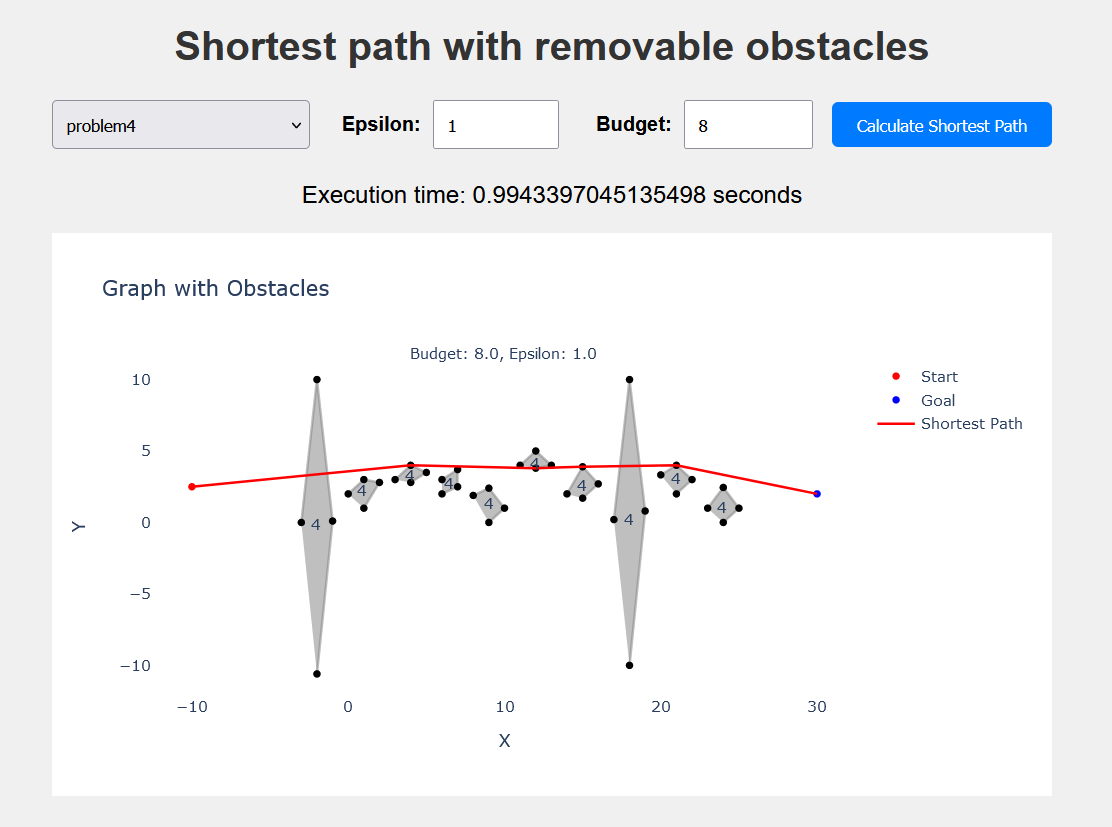
\includegraphics[width=1\textwidth]{web.png}
    \caption{Spletni vmesnik}
    \label{fig:web}
\end{figure}

Da bi lahko kasneje primerjal algoritme sem nekaj problemov tudi generiral. Sedaj lahko primerjam samo različna algoritma za konstrukcijo viability grapha, ter kako se potem počasnejši algoritem za iskanje poti obnaša ko manjšam $\epsilon$.

\begin{table}[h]
    \centering
    \begin{tabular}{|c|c|c|c|c|}
        \hline
        & \multicolumn{4}{c|}{n (število oglišč)} \\
        \cline{2-5}
        & 40 & 180 & 360 & 860 \\
        \hline
        Naivni algoritem & 0.5s & 36s &  301s &  1ura 47min\\
        \hline
        Sweep algoritem & 1s & 60s & 480s  & 1ura 51min \\
        \hline
    \end{tabular}
    \caption{Primerjava algoritmov za viability graph}
    \label{tab:1}
\end{table}

Oba algoritma bi morala imeti zahtevnost $O(n^3)$ in sweep se lepo ujema, naivni pa za velike $n$ hitreje upočasnjuje. Če bi bil $O(n^3)$ bi pričakoval za $n = 860$ pričakoval $(860/360)^3 \cdot 301s = 3900s = 65min$. Izgleda, da ima naivni algoritem zahtevnost $O(n^3 \log n)$, zato bi tudi tukaj bilo potrebno preverti implementacijo in razmisliti o izboljšavah. Upamo, da bosta do predstavitve algoritma hitrejša. Še primerjava za različne vrednosti $\epsilon$ pri $n=40$:

\begin{table}[h]
    \centering
    \begin{tabular}{|c|c|c|c|c|}
        \hline
        & \multicolumn{4}{c|}{$\epsilon$} \\
        \cline{2-5}
        & 0.01 & $10^{-3}$ & $10^{-4}$ & $10^{-5}$ \\
        \hline
        Naivni algoritem & 0.5s & 5s &  57s & memory full \\
        \hline
        Sweep algoritem & 1s & 11s & 126s  &  memory full \\
        \hline
    \end{tabular}
    \caption{Vpliv vrednosti $\epsilon$ na čas iskanja poti}
    \label{tab:2}
\end{table}

Algoritma sta v resnici čisto enaka, samo implementacija je malo drugačna. Pri naivnem oglišča grafa predstavim s slovarjem, ki ima za ključe cela števila, pri drugem grafu pa ključe pretvorim v tuple. To je edina razlika, ki jo opazim in zato mislim, da je razlog za to razliko. To je že druga priložnost za izboljšavo moje implementacije tega algoritma. Drugače pa kot pričakovano vidimo, da je zahtevnost $O(1/\epsilon)$.


\begin{thebibliography}{99}

    \bibitem{PNS} P.~K.~Agarwal, N.~Kumar, S.~Sintos in S.~Suri. \emph{Computing Shortest Paths in the Plane with Removable Obstacles}. 16. Scand. Symp. Work. Alg. Th. \textbf{101}, (2018);
    dostopno tudi na \url{https://drops.dagstuhl.de/entities/document/10.4230/LIPIcs.SWAT.2018.5}


    \bibitem{BCKO} M.~Berg, O.~Cheong, M.~Kreveld in  M.~Overmars \emph{Computational Geometry: Algorithms and Applications} Springer Berlin, Heidelberg, 2010

    \bibitem{SnT} N.~Sarnak in R.~E.~Tarjan \emph{Planar point location using persistent search trees}, Commun. ACM \textbf{29} (1986) 669-679; dostopno tudi na \url{https://dl.acm.org/doi/pdf/10.1145/6138.6151}

\end{thebibliography}
\end{document}

